\section{Metodo di lavoro}

Per lo sviluppo del progetto, in accordo con il tutor aziendale, è stata adottata una modalità di lavoro ibrida: 1–2 giorni alla settimana in presenza e il resto in remoto, 
con l'obiettivo di integrarmi nell'ambiente del \emph{team} che utilizza la stessa organizzazione. Per la comunicazione sincrona e asincrona ho impiegato 
\emph{Slack} per le interazioni quotidiane col tutor aziendale (richieste di chiarimenti, notifiche di avanzamento, condivisione di link e documenti) e per confermare i giorni di presenza 
della settimana successiva; per il lavoro in presenza ho utilizzato il mio PC portatile predisposto con l'ambiente di sviluppo richiesto dal progetto.

Il metodo di lavoro è stato concordato con il tutor aziendale attraverso un confronto iniziale e successive definizioni condivise: alcune parti del 
flusso mi sono state illustrate, altre sono state discusse e adattate tenendo conto delle mie osservazioni e competenze. Il processo complessivo è stato organizzato 
in fasi sequenziali e iterative; per ogni fase era previsto il rilascio di uno o più artefatti documentali e/o \emph{software} a supporto della valutazione e della 
verifica da parte del tutor aziendale. In particolare i \emph{deliverables} richiesti sono stati: documento di analisi del dominio (dimostrato anche tramite un \emph{playground} 
personale con esperimenti sulle tecnologie), documento di scelta tecnologica, specifica tecnica per il \emph{Proof of Concept} (\emph{PoC}) e la \emph{repository} ordinata 
con relativo \texttt{\emph{README.md}}.

\begin{figure}[H]
    \centering
    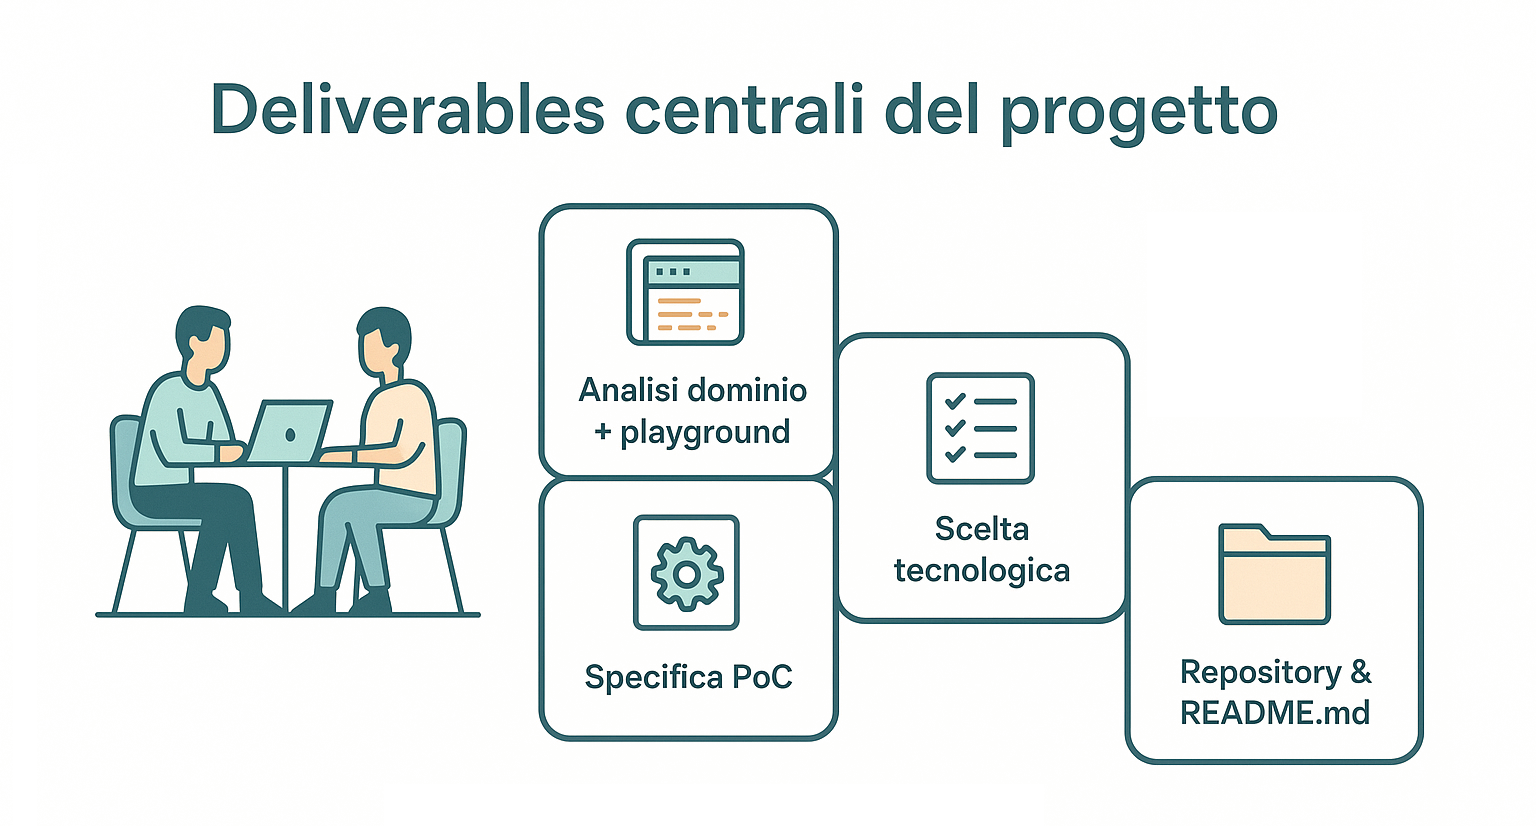
\includegraphics[width=0.8\textwidth]{stage/metodo}
    \caption{Schema del metodo di lavoro adottato.}
    \label{fig:metodo}
\end{figure}

Per garantire controllo, tracciabilità e qualità, ho seguito le pratiche sotto elencate, applicandole coerentemente alle attività giornaliere e alle revisioni settimanali:

\medskip
\noindent\textbf{Pianificazione e gestione delle attività}
Il progetto è stato pianificato in \emph{milestone} e \emph{task}: ogni \emph{milestone} conteneva obiettivi funzionali chiari e criteri di accettazione. 

\medskip
\noindent\textbf{Interazioni e revisioni con il tutor aziendale}
È stata stabilita una cadenza settimanale di incontro (giorno concordato di settimana in settimana) in cui presentare i progressi; 
ogni riunione seguiva un ordine del giorno strutturato: stato di avanzamento, dimostrazione pratica (se applicabile), punti aperti e rischi e proposte di soluzione.

\medskip
\noindent\textbf{Tracciamento dei requisiti e tecniche di analisi}
Ho adottato una procedura di tracciamento dei requisiti che mantenesse la relazione tra requisiti, attività di sviluppo e \emph{test}. 
Questo è stato realizzato tramite una semplice matrice di tracciabilità che associa ad ogni requisito: descrizione, priorità, \emph{task}/\emph{issue} corrispondenti.

\medskip
\noindent\textbf{Controllo della qualità del software e strumenti di verifica}
Per il codice ho seguito pratiche consolidate: utilizzo di controllo versione 
(\emph{git}) con flusso a \emph{feature-branch} e \emph{linters/formatter} per mantenere qualità e uniformità. 
Ho predisposto \emph{test} manuali per i componenti critici, per le \emph{API} e le varie integrazioni. 
Per la verifica funzionale del PoC sono stati definiti casi di \emph{test} che verificano il rispetto dei requisiti definiti nel relativo documento.

\medskip
\noindent\textbf{Sicurezza e gestione dei dati}
Per le integrazioni con \emph{API} esterne (Shopify e Sanity) e per qualsiasi dato sensibile ho rispettato accorgimenti base: 
uso di variabili d'ambiente, non salvataggio di chiavi in chiaro e repository privata con accesso consentito solamente al tutor aziendale.

\medskip
\noindent\textbf{Documentazione e repository}
La repository del progetto è stata organizzata con una struttura logica (cartelle per codice, \emph{test} e documentazione) 
e corredata da un \texttt{\emph{README.md}} esaustivo che spiega come eseguire il progetto, come riprodurre il \emph{PoC} e quali sono i componenti principali.


%interazioni con il tutor aziendale



%Sezione che riporterà il flusso di lavoro uilizzato per lo sviluppo del progetto in accordo con il tutor aziendale.
%Verranno riportati pianificazione, interazioni con il tutor aziendale, revisioni di progresso, uso di diagrammi,
%tecniche di analisi e tracciamento dei requisiti, strumenti di verifica, ecc.
%Qui descriverò il punto 3.a (cosa e come) riportato nel file Struttura relazione finale.pdf.
